\chapter{Algebraic Diagrammatic Construction (ADC)}
\section{One-Particle-Greensfunctions}\label{greensfkt}

Green's function methods are based on propagators, which contain information
about the response of a system to a time-dependent perturbation.\cite{McWeeny89}
They are advantageous compared to other quantum chemical methods, because they
allow the calculation of properties like energy differences without calculating
the two different states but instead calculating their difference directly.

In the time-domain, the propagator, also called the one particle Green's function
for fermions is defined as

\begin{equation}\label{1pgf}
G_{pq}(t,t') = -i \bra{\Psi_0^N}c_p(t)c_q^\dagger(t')\ket{\Psi_0^N}\Theta(t-t') +i \bra{\Psi_0^N}c_q^\dagger(t')c_p(t)\ket{\Psi_0^N}\Theta(t'-t)
\end{equation}

Here, $\Theta(t-t')$ is the Heaviside step function eq. (\ref{stufe}),
which ensures the causality of the described process. A system can only
respond to a perturbation which occured in the past. Therefore, the Green's
function is non-zero for times $t>t'$ and zero for all other times. \cite{nolting7}

\begin{equation}\label{stufe}
\Theta(t-t') = \begin{cases}
1 & \text{for } t>t'\\
0 & \text{for } t<t'
\end{cases}
\end{equation}

In the non-Dyson formulation \cite{Schirmer89} the Green's function can be
written as the sum over the $N+1$ and the $N-1$ parts

\begin{equation}
G_{pq}(\omega) = G_{pq}^+(\omega) + G_{pq}^-(\omega)
\end{equation}

The Green's functions are formulated in the Heisenberg picture, where the
operators are time-dependent and the states are time-independent.
The annihilation and creation operators are therefore defined as
$c_p(t) = \mathrm{e}^{-i\mathcal{H} t} c_p \mathrm{e}^{i\mathcal{H} t}$.
Inserting these into the $N-1$ part of equation (\ref{1pgf}) yields


\begin{equation}\label{g-hsb}
G_{pq}^-(t',t) = i\Theta(t'-t) \mathrm{e}^{iE_0^N(t'-t)}\bra{\Psi_0^N}c_q^\dagger\mathrm{e}^{-i\mathcal{H}(t'-t)}c_p\ket{\Psi_0^N}
\end{equation}
For a time-independent Hamilton operator $\mathcal{H}$ the Green's function
depends only on the time difference $t'-t$ and therefore $G_{pq}(t',t)$ is
transformed into $G_{pq}(t'-t)$. The $N+1$ part is treated analogously.

After insertion of a complete $N+1$ basis $\ket{\Psi_n^{N-1}}$ in
$G_{pq}^+$ and $N-1$ basis $\ket{\Psi_n^{N-1}}$
into $G_{pq}^-$ the Green's function is Fourier transformed from the time
into the energy domain. To ensure the convergence, 
$\mathrm{e}^{-\eta(t'-t)}$ or $\mathrm{e}^{-\eta(t-t')}$ are introduced,
where $\eta$ is infinitesimal and positive.
This yields the spectral representation

\begin{equation}\label{spektraldst}
G_{pq}(\omega) = \sum\limits_{n\in\{N+1\}}\frac{x_p^{(n)}x_q^{(n)*}}{\omega-e_n +i\eta} + \sum\limits_{n\in\{N-1\}}\frac{x_p^{(n)}x_q^{(n)*}}{\omega-e_n -i\eta}
\end{equation}

with $e_n$ being the energy differences between initial and final state. Hence,
in case of the one particle propagator, the poles of the Green's function
are the ionization energies and electron affinities.
The pole strengths $\left|x_p^{(n)}\right|^2$ correspond to the transition
probability and are the square of the transition amplitudes
$x_p^{(n)}=\bra{\Psi_n^{N-1}}c_p\ket{\Psi_0}$.



\section{Two Particle Green's function}
Analog to the the one particle Green's function, the two particle Green's
function $\mathbf{\Pi}(\omega)$ describes the process of double ionization
or electron attachment. Its poles again correspond to the ionization energies
and electron affinities.

\begin{equation}
\mathbf{\Pi}_{\alpha\beta,\alpha'\beta'}(\omega) = \sum\limits_{m\in N+2} \frac{x^{(m)}_{\alpha\beta}x^{*(m)}_{\alpha'\beta'}}{\omega +E_0^N-E_n^{N+2}+i\eta} - \sum\limits_{m\in N-2} \frac{x^{(m)}_{\alpha\beta}x^{*(m)}_{\alpha'\beta'}}{\omega +E_m^{N-2}-E_0^{N}-i\eta}
\end{equation}

Here the transition amplitudes are given by
\begin{equation}
x^{(m)}_{\alpha\beta}=\begin{cases}
\braket{\Psi_0^N|a_\alpha a_\beta|\Psi_n^{N+2}} & \text{for } m\in N+2\\
\braket{\Psi_n^{N-2}|a_\alpha a_\beta|\Psi_0^{N}} & \text{for } m\in N-2,
\end{cases}
\end{equation}

where $a_\alpha$ and $a_\beta$ are the annihilation and creation operators of
the orbitals $\alpha$ and $\beta$, respectively.



\section{\acl{ADC}}
Originally the Green's function was formulated in the Dyson ansatz and
determined using perturbation theory. This way both the ionization and the
electron affinity part had to be included in the description. In the non-Dyson
scheme those two are separable and hence the dimension of the problem is reduced
when one is interested in either the $N+1$ or the $N-1$ part. \cite{Schirmer98}
The ionization part $\mathbf{G^-}(\omega)$ is transposed to give
$\tilde{G}_{pq}(\omega) = G^-_{qp}(\omega)$. From this, the compact matrix
form can be deduced

\begin{equation}\label{matrixspec}
\mathbf{\tilde{G}}(\omega) = \mathbf{x}^\dagger(\omega-\mathbf{\Omega})^{-1}\mathbf{x}
\end{equation}

To this point, the problem is exact. However, the exact wavefunctions are unknown
and hence the basis of so-called \emph{intermediate states} are introduced. These
are formally constructed from \ac{CES} as they appear in a
\ac{CI} expansion. These \ac{CES} are then grouped into excitation classes
and these classes are orthogonalized with respect to each other. Afterwards,
the states within each class are orthogonalized. 
This approach has the advantage to be size-consistent and hence
suiTable for the description of larger systems. \cite{Mertins96_1}

In this \ac{ISR} the Green's function can be written as
\begin{equation}\label{isradc}
\mathbf{\tilde{G}}(\omega) = \mathbf{f}^\dagger(\omega-\mathbf{K}-\mathbf{C})^{-1}\mathbf{f}
\end{equation}

Here, $\mathbf{K}$ is the diagonal matrix of Hartree Fock orbital energies, which
corresponds to zeroth order of perturbation theory. The matrix $\mathbf{C}$
contains all higher order contributions to the Hamiltonian.
Hence, the ADC matrix $\mathbf{M} = \mathbf{K}+\mathbf{C}$ is non-diagonal.
This equation can be solved by
solving the eigenvalue problem

\begin{equation}\label{adcewp}
(\mathbf{K}+\mathbf{C}) \mathbf{Y} = \mathbf{Y}\mathbf{\Omega} \quad\text{where } \mathbf{Y}^\dagger\mathbf{Y}=\mathbf{1}
\end{equation}
where $\mathbf{\Omega}$ is the matrix of eigenvalues and hence the ionization
energies and $\mathbf{Y}$ is the matrix of eigenvectors which connects the
intermediate state representation with the exact $N-1$ solutions.

\begin{equation}
 \mathbf{x} = \mathbf{Y}^\dagger \mathbf{f}
\end{equation}

For the construction of the \ac{ADC} matrix ($\mathbf{K}+\mathbf{C}$) and the
effective transitions moments $\mathbf{f}$, $\mathbf{C}$ and $\mathbf{f}$
are expanded into different orders of perturbations and inserted to equation
(\ref{isradc}).

\begin{eqnarray}
\mathbf{C} &=& \mathbf{C}^{(1)} + \mathbf{C}^{(2)} + \mathbf{C}^{(3)} + \cdots\label{stC}\\
\mathbf{f} &=& \mathbf{f}^{(0)} + \mathbf{f}^{(1)} + \mathbf{f}^{(2)} + \cdots\label{stf}
\end{eqnarray}

From this, different orders of perturbation theory of the Hamiltonian can be
constructed successively. The contributions to the different classes are shown
in Figure \ref{figure:adcmat_pgf} for the case of \ac{ADC}(2x).

\begin{figure}[h]
  \centering
  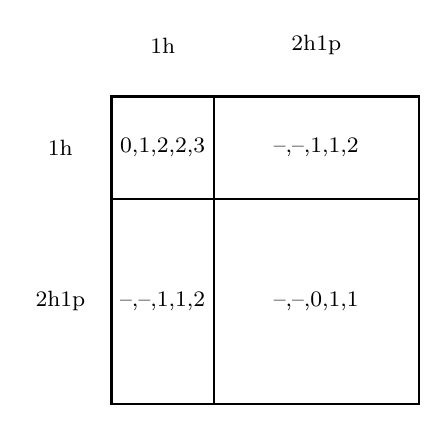
\begin{tikzpicture}[scale=1.3]
    \footnotesize
    %\draw [help lines] (-1,0) grid (23,5);
    \draw [thick] (0,0) rectangle (3,3);
    \draw [thick] (0,2) rectangle (1,3) node [midway] {0,1,2,2,3};
    \draw [thick] (1,0) rectangle (3,2) node [midway] {--,--,0,1,1};
    \draw [thick] (0,0) rectangle (1,2) node [midway] {--,--,1,1,2};
    \draw [thick] (1,2) rectangle (3,3) node [midway] {--,--,1,1,2};
    \node (1h1) at (0.5,3.5) {1h};
    \node (1h2) at (-0.5,2.5) {1h};
    \node (2h1) at (2.0,3.5) {2h1p};
    \node (2h2) at (-0.5,1.0) {2h1p};

\end{tikzpicture}

  \caption{Schematic illustration of an \ac{ADC}(2x) matrix.}
  \label{figure:adcmat_pgf}
\end{figure}

The matrix elements are explicitely given by
\begin{itemize}
 \item 1h/1h (1h block):
   \begin{align}
    M_{kk'}^{(0)} &= \varepsilon_k \delta_{kk'} \\
    M_{kk'}^{(1)} &= 0 \\
    M_{kk'}^{(2)} &= -\frac12 \sum\limits_{abl} V_{ab[kl]} V_{k'l[ab]} %\times
                     \frac{\varepsilon_a+\varepsilon_b-\varepsilon_l
                       -\frac12 \varepsilon_k-\frac12 \varepsilon_{k'}}
                     {(\varepsilon_a+\varepsilon_b-\varepsilon_k-\varepsilon_l)
                      (\varepsilon_a+\varepsilon_b-\varepsilon_{k'}-\varepsilon_l)}
   \end{align}
 \item 1h/2h1p (coupling block):
   \begin{equation}
    M_{j,akl}^{(1)} = V_{kl[aj]}
   \end{equation}
 \item 2h1p/2h1p (satellite block):
   \begin{align}
    M_{akl,a'k'l'}^{(0)} &= (-\varepsilon_a+\varepsilon_k+\varepsilon_l)
                             \, \delta_{aa'}\delta_{kk'}\delta_{ll'} \\
    M_{akl,a'k'l'}^{(1)} &= -\delta_{aa'} V_{k'l'[kl]} + \delta_{kk'} V_{al'[a'l]}
                            +\delta_{ll'} V_{ak'[a'k]} - (k \leftrightarrow l)
   \end{align}
\end{itemize}

Here, $\varepsilon$ denotes the Hartree Fock energy. The occupied states are labelled
by $i,j,k,\dots$ and the unoccupied states are labelled by $a,b,c,\dots$. The
two-electron integrals for any combination of occupied and unoccupied orbitals
labelled by $p,q,r,s$ read as
\begin{equation}
 V_{pqrs} = \braket{\varphi_p(1)\varphi_q(2) |V(1,2)| \varphi_r(1)\varphi_s(2)}
\end{equation}

and $V_{pq[rs]} = V_{pqrs} - V_{pqsr}$.

